\documentclass[12pt]{article}
\input{preamble}

\pagestyle{fancy}
\fancyhf{}

\rhead{Nørre G \\
1.g
}


%Husk at rette modul og dato!
\lhead{Matematik A\\
	Komplekse tal
}
\chead{
}

\cfoot{Side \thepage \hspace{1pt} af \pageref{LastPage}}

\begin{document}

%Udfyld afsnit herunder og lav til egen Latex-fil

%Kopier følgende til overskrift:

%\begin{center}
%\Huge
%Aflevering 1
%\end{center}
%\section*{Opgave 1}
%\stepcounter{section}
%Overskrift

%\begin{center}
%\Huge
%Aflevering 1
%\end{center}


\begin{center}
	\Huge
	Eulers formel og polære repræsentationer
\end{center}
\stepcounter{section}
Vi så sidst, at komplekse tal på polær form opfører sig som eksponentialfunktioner, når vi ganger dem sammen. Dette viser sig ikke at være tilfældigt. Én af de mest bemærkelsesværdige resultater med komplekse tal er det, vi kalder \textit{Eulers formel}.
\begin{setn}[Eulers formel]
	For ethvert tal $x \in \mathbb{R}$ gælder der, at 
	\begin{align*}
		e^{ix} = \cos(x) + i\sin(x).
	\end{align*}
\end{setn}
Vi vil senere bevise, at dette er sandt, men det har vi desværre ikke værktøjet til endnu. Vi vil dog som et eksempel på ligningens anvendelse vise et andet ganske berømt resultat.
\begin{exa}
	Indsættes $x = \pi$ i Eulers formel, får vi
	\begin{align*}
		e^{\pi i} = \cos(\pi) + i \sin(\pi) = -1 + i\cdot 0 = -1,
	\end{align*}
	altså at $e^{\pi i } = -1$. Det er pænt overraskende, at tre konstanter $e$, $\pi$ og $i$, der er defineret i tre 
	forskellige grene af matematikken viser sig at have dette indbyrdes forhold. 
\end{exa}
Vi kan også bruge Eulers formel til at skrive komplekse tal på polær form. Vi husker, at et komplekst tal på polær form er givet ved
\begin{align*}
	z = r(\cos(\theta)+ i \sin(\theta)).
\end{align*}
Vi må derfor kunne skrive
\begin{align*}
	z &= r(\cos(\theta)+ i \sin(\theta))\\
	&=re^{i\theta}.
\end{align*}
Dette gør altså, at vi ikke skal bruge $\cis$-notationen, men blot kan bruge denne repræsentation for det komplekse tal. 
Lad os betragte et par eksempler.
\begin{exa}
	Vi ønsker at repræsentere tallet $z = 1 - i$ på formen $re^{i\theta}$. Vi bestemmer modulus $r$ og argumentet 
	$\theta$ som tidligere. Først modulus.
	\begin{align*}
		r &= |z| = \sqrt{1^2 + (-1)^2} = \sqrt{2}.
	\end{align*}
	Nu argumentet.
	\begin{align*}
		\tan(\theta) = \frac{-1}{1} = -1.
	\end{align*}
	Da $z$ ligger i 4. kvadrant, får vi at $\theta = \frac{7\pi}{4}$. 
	Vi kan derfor skrive vores komplekse tal $z$ som
	\begin{align*}
		z = \sqrt{2}e^{i \frac{7 \pi}{4}}
	\end{align*}
\end{exa}	
\begin{exa}
	Vi har fået det komplekse tal 
	\begin{align*}
		z = 3e^{-i\frac{5\pi}{6}}
	\end{align*}
	og vil gerne have det på formen $z = a + bi$. Vi husker på, at vi kan skrive $z$ som
	\begin{align*}
		z = 3\left(\cos\left(\frac{-5\pi}{6}\right) + i \sin\left(\frac{-5\pi}{6}\right)\right)
	\end{align*}
	Vi skal altså have fundet vores realdel som 
	\begin{align*}
		3\cos\left(\frac{-5\pi}{6}\right),
	\end{align*}
	og vores imaginærdel som
	\begin{align*}
		3\sin\left(\frac{-5\pi}{6}\right).
	\end{align*}
	Vi anvender den altid brugbare Tabel \ref{tab:trig} samt enhedscirklen på Figur \ref{fig:enhed}.
	Vi får så, at 
	\begin{align*}
		3\cos\left(\frac{-5\pi}{6}\right) = 3\cdot \frac{-\sqrt{3}}{2} = \frac{-3\sqrt{3}}{2}
	\end{align*}
	og 
	\begin{align*}
		3\sin\left(\frac{-5\pi}{6}\right) = 3\cdot \frac{-1}{2} = \frac{-3}{2}.
	\end{align*}
	Det komplekse tal på formen $z = a + bi$ lyder derfor
	\begin{align*}
		z = -\frac{3\sqrt{3}}{2} - \frac{3}{2}i.
	\end{align*}
\end{exa}
\begin{table}[H]
	\centering
	\rowcolors{1}{SeaGreen!20}{Melon!20}
	\begin{tabular}{cccccc}
		$\theta$ & 0 & $\frac{\pi}{6}$ & $\frac{\pi}{4}$ & $\frac{\pi}{3}$ & $\frac{\pi}{2}$ \\
		$\cos(\theta)$ & 1 &  $\frac{\sqrt{3}}{2}$ & $\frac{\sqrt{2}}{2}$ & $\frac{1}{2}$ & 0 \\
		$\sin(\theta)$ & 0 & $\frac{1}{2}$ & $\frac{\sqrt{2}}{2}$ &  $\frac{\sqrt{3}}{2}$ & 1 \\
		$\tan(\theta)$ & 0 &  $\frac{\sqrt{3}}{3}$ & 1 & $\sqrt{3}$ & 
	\end{tabular}
	\caption{Vigtige funktionsværdier for cos, sin og tan.}
	\label{tab:trig}
\end{table}
\begin{figure}[H]
	\centering
	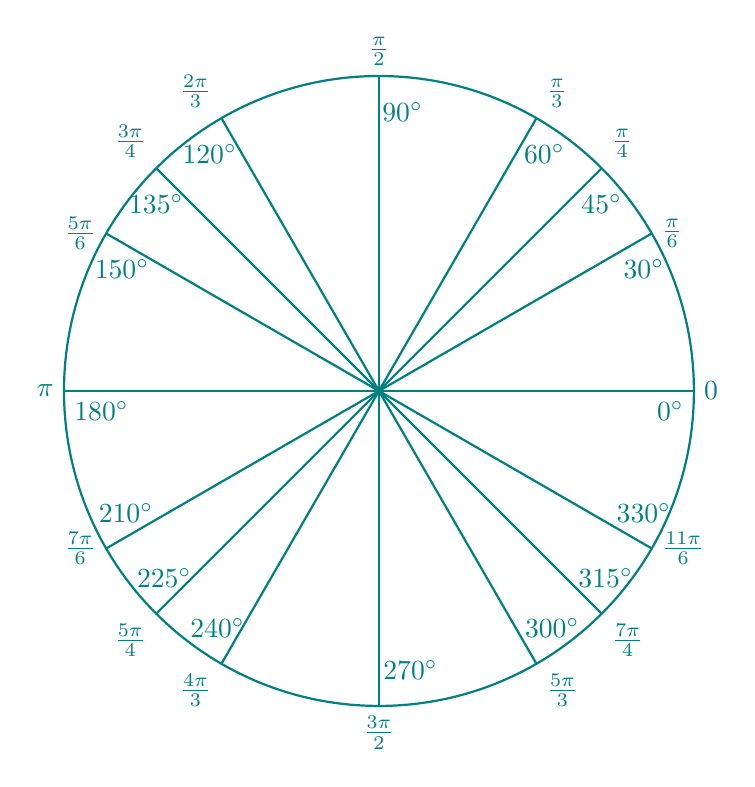
\begin{tikzpicture}
		\draw[thick, color = teal] (0,0) circle (4cm);
		\draw[thick, color = teal] (0,0) -- ({4*cos(0)},{4*sin(0)})
		node[pos = 1, anchor = north east] {$0^\circ$}
		node[pos = 1, anchor = west] {0};
		\draw[thick, color = teal] (0,0) -- ({4*cos(30)},{4*sin(30)})
		node[pos = 1, anchor = north, yshift = -0.2cm, xshift = -0.1cm] {$30^\circ$}
		node[pos = 1, anchor = west] {$\frac{\pi}{6}$};
		\draw[thick, color = teal] (0,0) -- ({4*cos(45)},{4*sin(45)})
		node[pos = 1, anchor = north, yshift = -0.2cm, xshift = -0cm] {$45^\circ$}
		node[pos = 1, anchor = south west] {$\frac{\pi}{4}$};
		\draw[thick, color = teal] (0,0) -- ({4*cos(60)},{4*sin(60)})
		node[pos = 1, anchor = north, yshift = -0.2cm, xshift = 0.1cm] {$60^\circ$}
		node[pos = 1, anchor = south west] {$\frac{\pi}{3}$};
		\draw[thick, color = teal] (0,0) -- ({4*cos(90)},{4*sin(90)})
		node[pos = 1, anchor = north, yshift = -0.2cm, xshift = 0.3cm] {$90^\circ$}
		node[pos = 1, anchor = south] {$\frac{\pi}{2}$};
		\draw[thick, color = teal] (0,0) -- ({4*cos(120)},{4*sin(120)})
		node[pos = 1, anchor = north, yshift = -0.2cm, xshift = -0.15cm] {$120^\circ$}
		node[pos = 1, anchor = south east] {$\frac{2\pi}{3}$};
		\draw[thick, color = teal] (0,0) -- ({4*cos(135)},{4*sin(135)})
		node[pos = 1, anchor = north, yshift = -0.2cm, xshift = -0cm] {$135^\circ$}
		node[pos = 1, anchor = south east] {$\frac{3\pi}{4}$};
		\draw[thick, color = teal] (0,0) -- ({4*cos(150)},{4*sin(150)})
		node[pos = 1, anchor = north, yshift = -0.2cm, xshift = 0.2cm] {$150^\circ$}
		node[pos = 1, anchor = east] {$\frac{5\pi}{6}$};
		\draw[thick, color = teal] (0,0) -- ({4*cos(180)},{4*sin(180)})
		node[pos = 1, anchor = north west] {$180^\circ$}
		node[pos = 1, anchor = east] {$\pi$};
		\draw[thick, color = teal] (0,0) -- ({4*cos(210)},{4*sin(210)})
		node[pos = 1, anchor = south, yshift = 0.2cm, xshift = 0.25cm] {$210^\circ$}
		node[pos = 1, anchor = east] {$\frac{7\pi}{6}$};
		\draw[thick, color = teal] (0,0) -- ({4*cos(225)},{4*sin(225)})
		node[pos = 1, anchor = south, yshift = 0.2cm, xshift = 0.1cm] {$225^\circ$}
		node[pos = 1, anchor = north east] {$\frac{5\pi}{4}$};
		\draw[thick, color = teal] (0,0) -- ({4*cos(240)},{4*sin(240)})
		node[pos = 1, anchor = south, yshift = 0.2cm, xshift = -0.05cm] {$240^\circ$}
		node[pos = 1, anchor = north east] {$\frac{4\pi}{3}$};
		\draw[thick, color = teal] (0,0) -- ({4*cos(270)},{4*sin(270)})
		node[pos = 1, anchor = south, yshift = 0.2cm, xshift = 0.4cm] {$270^\circ$}
		node[pos = 1, anchor = north] {$\frac{3\pi}{2}$};
		\draw[thick, color = teal] (0,0) -- ({4*cos(300)},{4*sin(300)})
		node[pos = 1, anchor = south, yshift = 0.2cm, xshift = 0.2cm] {$300^\circ$}
		node[pos = 1, anchor = north west] {$\frac{5\pi}{3}$};
		\draw[thick, color = teal] (0,0) -- ({4*cos(315)},{4*sin(315)})
		node[pos = 1, anchor = south, yshift = 0.2cm, xshift = 0.05cm] {$315^\circ$}
		node[pos = 1, anchor = north west] {$\frac{7\pi}{4}$};
		\draw[thick, color = teal] (0,0) -- ({4*cos(330)},{4*sin(330)})
		node[pos = 1, anchor = south, yshift = 0.2cm, xshift = -0.1cm] {$330^\circ$}
		node[pos = 1, anchor = west] {$\frac{11\pi}{6}$};
	\end{tikzpicture}
	\caption{Enhedscirklen med udvalgte vigtige vinkler.}
	\label{fig:enhed}
\end{figure}

\subsection*{Opgave 1}
Skriv følgende komplekse tal på formen $re^{i\theta}$. 
\begin{align*}
	&1) \ -1   &&2) \ -i - 1   &&3) \  \sqrt{3} - i   \\
	&4) \ \frac{1 + i}{2}   &&5) \ \sqrt{2} - \sqrt{2}i   &&6) \  3 - 3\sqrt{3}i     \\
	&7) \ (1-i)^5   &&8) \ 7\cis(5\pi/11)   &&9) \ \frac{1}{i}     \\
\end{align*}

\subsection*{Opgave 2}
Omskriv følgende komplekse tal på formen $a + bi$
\begin{align*}
	&1) \ e^{i\pi/3}  &&2) \ 2e^{-5\pi i/6}   &&3) \  5e^{i 11\pi/12}   \\
	&4) \ \sqrt{2}(e^{i \pi/3})^7   &&5) \ 7e^{-\pi i / 2 }   &&6) \   4\sqrt{e^{i 3\pi/2}}    \\
\end{align*}

\subsection*{Opgave 3}
Vi kan definere $\cos$ og $\sin$ ud fra den komplekse eksponentialfunktion på følgende måde
\begin{align*}
	\cos(\theta) = \frac{e^{i\theta}+e^{-i\theta}}{2}
\end{align*}
og
\begin{align*}
	\sin(\theta) = \frac{e^{i\theta}-e^{-i\theta}}{2i}
\end{align*}
\begin{enumerate}[label=\roman*)]
	\item Vis, at denne definition stemmer overens med definitionen af $\cos$ og $\sin$ ved at bruge Eulers formel på 
	leddene i tælleren. 
\end{enumerate}
\subsection*{Opgave 4}
Vi har følgende trigonometriske identiteter, der ofte er brugbare. Disse er lidt mere ligetil at bevise, når vi har disse formler fra Opgave 3.
\begin{enumerate}[label=\roman*)]
	\item Vis, at $\cos(v + w) = \cos(v)\cos(w) - \sin(v)\sin(w)$ ved at bruge udtrykket for $\cos$ og $\sin$ fra
	 Opgave 3 på højresiden i udtrykket.
	\item Vis, at $\sin(v + w) = \sin(v)\cos(w) + \cos(v)\sin(w)$ ved at bruge udtrykket for $\cos$ og $\sin$ fra 
	Opgave 3 på højresiden i udtrykket. 
	
\end{enumerate}

\newpage

\begin{center}
	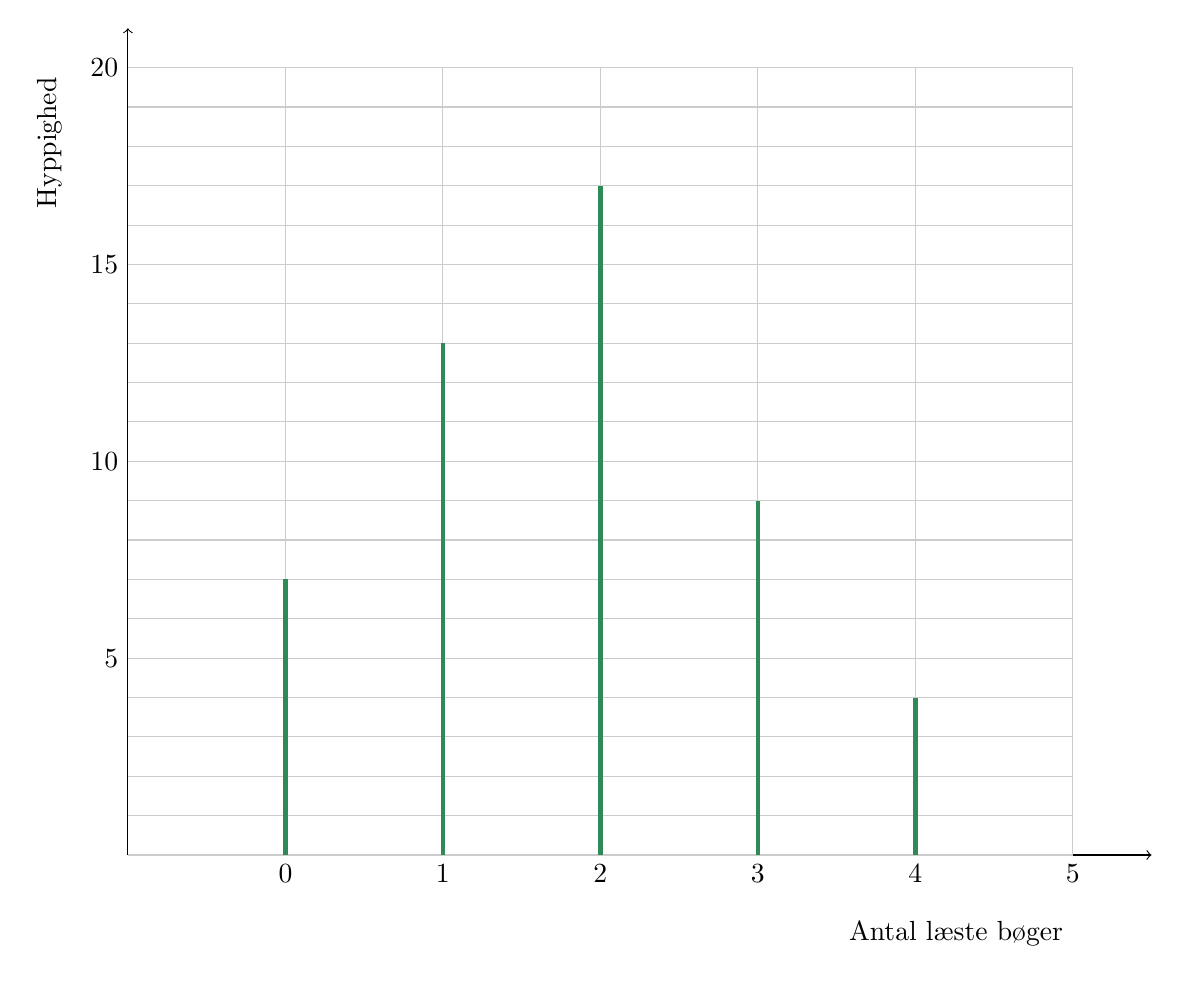
\begin{tikzpicture}
	\draw[->] (1,1) -- (14,1);
	\draw[->] (1,1) -- (1,11.5);
	\foreach \x in {0,1,2,3,4,5}{
		\draw[thin, color = gray!40] ({2*\x + 3}, 1) -- ({2*\x + 3}, 11);
		\node[anchor = north] at ( {2*\x + 3}, 1) {$\x $};
	}
	\foreach \x in {0,1,...,20}{
		\draw[thin, color = gray!40] (1,{0.5*\x + 1}) -- (13,{0.5*\x + 1});
	}
	\foreach \x in {5,10,15,20}{
		\node[anchor = east] at (1, {0.5*\x + 1}) {$\x$};
	}
	\draw[color = SeaGreen, ultra thick] (3,1) -- (3, 4.5);
	\draw[color = SeaGreen, ultra thick] (5,1) -- (5, 7.5);
	\draw[color = SeaGreen, ultra thick] (7,1) -- (7, 9.5);
	\draw[color = SeaGreen, ultra thick] (9,1) -- (9, 5.5);
	\draw[color = SeaGreen, ultra thick] (11,1) -- (11, 3);
	\node[anchor = east] at (13,0) {Antal læste bøger};
	\node[anchor = east, rotate = 90] at (0,11) {Hyppighed};
	\end{tikzpicture}
\end{center}
\end{document}